% Chapter 3 -- Motion in a central potential; the Kepler problem.
%
% Reference convention: Goldstein, Poole & Safko, "Classical
% Mechanics," 3rd ed., Ch. 3 "The Central Force Problem", adopted for
% terminology and equation style. Symbols follow this document's own
% declarations below, which govern wherever they differ from Goldstein's.

\documentclass[11pt]{article}
\usepackage{goldsteinnotes}
\usepackage{tikz}
\usepackage{cancel}
\usepackage{sectsty}
\usetikzlibrary{arrows.meta,calc}

\allsectionsfont{\boldmath}

% Numbering carries the chapter, so sections and equations read 3.n.
\renewcommand{\thesection}{3.\arabic{section}}
\renewcommand{\theequation}{3.\arabic{equation}}
\renewcommand{\thefigure}{3.\arabic{figure}}

% --- symbols fixed for THIS document (see the scope note in goldsteinnotes.sty)
% mu   : reduced mass
% \ell : conserved angular momentum, the magnitude of \vec{L}
% phi  : azimuthal angle in the plane of motion
% u = 1/r,  V = -k/r,  e = eccentricity
% Vectors carry arrows and unit vectors carry hats, as declared here.
\renewcommand{\vect}[1]{\vec{#1}}
\renewcommand{\unit}[1]{\hat{#1}}

% The aside is ruled off from the surrounding argument.
\newenvironment{asidebox}
  {\par\addvspace{6pt}\hrule\addvspace{5pt}\noindent\textit{Aside.}\ }
  {\par\addvspace{5pt}\hrule\addvspace{7pt}}

\title{\textbf{Chapter 3}\\[2pt] Motion in Central Potential $V(r)$}
\author{}
\date{}

\begin{document}
\maketitle
\vspace{-2.5em}

\section{Angular momentum and the Lagrangian}

\begin{equation}
  \vect{L} = \mu r^{2}\dot{\phi}\,\unit{z},
  \qquad \vect{r} = r\,\unit{r},
  \qquad \vect{p} = \mu\dot{\vect{r}},
\end{equation}
with $\vect{L}$ a constant of the motion. The Lagrangian is
\begin{equation}
  L = T - V = \frac{\mu}{2}\left(\dot{r}^{2} + r^{2}\dot{\phi}^{2}\right) - V(r).
\end{equation}

Since $\phi$ is cyclic,
\begin{equation}
  \pd{L}{\phi} = 0
  \quad\Longrightarrow\quad
  p_{\phi} = \pd{L}{\dot{\phi}} = \mu r^{2}\dot{\phi} \equiv \ell
  \quad \text{conserved}.
\end{equation}

The effective potential and the energy are
\begin{align}
  V_{\text{eff}}(r) &= V(r) + \frac{\ell^{2}}{2\mu r^{2}}, \\[4pt]
  E = T + V &= \frac{\mu}{2}\left(\dot{r}^{2} + r^{2}\dot{\phi}^{2}\right) + V(r)
            = \frac{\mu}{2}\dot{r}^{2} + V_{\text{eff}}(r).
\end{align}

\section{Universal method \texorpdfstring{$\Rightarrow$}{=>} complete solution}

\begin{equation}
  \boxeq{
  \begin{aligned}
    t &= \int_{r_{0}}^{r}
         \frac{\d r'}{\rule{0pt}{2.4em}\sqrt{\dfrac{2}{\mu}\left(E - V(r') - \dfrac{\ell^{2}}{2\mu r'^{2}}\right)}}\\[10pt]
    \phi &= \phi_{0} + \int_{t_{0}}^{t} \frac{\ell}{\mu r^{2}(t')}\,\d t'
  \end{aligned}}
  \qquad
  \begin{aligned}
    &t = t(r)
      \vphantom{\frac{\d r'}{\rule{0pt}{2.4em}\sqrt{\dfrac{2}{\mu}\left(E - V(r') - \dfrac{\ell^{2}}{2\mu r'^{2}}\right)}}}\\[10pt]
    &\phi = \phi(t)
      \vphantom{\int_{t_{0}}^{t}\frac{\ell}{\mu r^{2}(t')}}
  \end{aligned}
\end{equation}

\section{Differential equation for \texorpdfstring{$r = r(\phi)$}{r = r(phi)}}

\begin{equation}
  \ell = \mu r^{2}\dot{\phi}
  \quad\Longrightarrow\quad
  \dot{\phi} = \frac{\ell}{\mu r^{2}} = \dd{\phi}{t},
\end{equation}
so that for any $F$,
\begin{equation}
  \dd{F}{t} = \dd{F}{\phi}\,\dd{\phi}{t}
            = \underbrace{\frac{\ell}{\mu r^{2}}\,\dd{F}{\phi}}_{}\!.
  \label{eq:operator}
\end{equation}
The orbit is sketched in Fig.~\ref{fig:orbit}.

\begin{figure}[htbp]
  \centering
  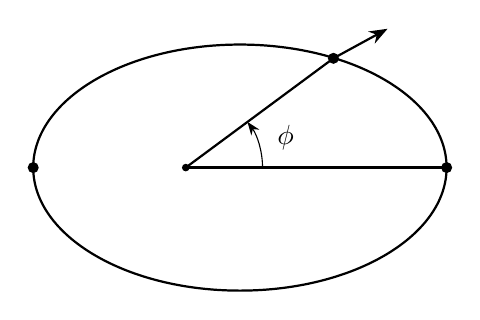
\begin{tikzpicture}[scale=1.25,>=Stealth]
    \draw[thick] (0,0) ellipse [x radius=2.1, y radius=1.25];
    \coordinate (O) at (-0.55,0);
    \coordinate (P) at (0.95,1.11);
    \coordinate (R) at (2.1,0);
    \fill (O) circle (1.1pt);
    \fill (R) circle (1.6pt);
    \fill (-2.1,0) circle (1.6pt);
    \fill (P) circle (1.6pt);
    \draw[thick] (O) -- (R);
    \draw[thick] (O) -- (P);
    \draw[->,thick] (P) -- ++(0.55,0.30);
    \draw[->] ($(O)+(0:0.78)$) arc [start angle=0, end angle=36.5, radius=0.78];
    \node at ($(O)+(17:1.06)$) {$\phi$};
  \end{tikzpicture}
  \caption{The orbit in the plane of motion.}
  \label{fig:orbit}
\end{figure}

With $-\pd{V}{r} = F(r)$, the radial equation of motion is
\begin{equation}
  \mu\ddot{r} = -\pd{V_{\text{eff}}}{r}
              = -\pd{}{r}\left(V(r) + \frac{\ell^{2}}{2\mu r^{2}}\right),
\end{equation}
and since $\pd{}{r}\left(r^{-2}\right) = (-2)r^{-3}$,
\begin{equation}
  \mu\ddot{r} = F(r) + \frac{\ell^{2}}{\mu r^{3}}.
\end{equation}

\section{The substitution \texorpdfstring{$u = 1/r$}{u = 1/r}}

Set
\begin{equation}
  u = \frac{1}{r},
  \qquad
  \dd{u}{\phi} = \dd{u}{r}\,\dd{r}{\phi} = -\frac{1}{r^{2}}\,\dd{r}{\phi}.
\end{equation}

Writing $F$ in $u$ as $F(1/u)$ (Sec.~\ref{sec:force}),
\begin{equation}
  \frac{\ell^{2}}{\mu r^{3}} = \frac{\ell^{2}}{\mu}u^{3}
  \quad\Longrightarrow\quad
  \text{RHS:}\;\; F(1/u) + \frac{\ell^{2}}{\mu}u^{3}.
\end{equation}

\paragraph{LHS:} applying Eq.~\eqref{eq:operator} twice,
\begin{equation}
  \mu\,\ddt{}\,\dd{r}{t}
    = \mu\,\ddt{}\,\frac{\ell}{\mu r^{2}}\,\dd{r}{\phi}
    = \,\cancel{\mu}\,\frac{\ell}{\cancel{\mu}\, r^{2}}\,\dd{}{\phi}
      \left(\frac{\ell}{\mu r^{2}}\,\dd{r}{\phi}\right).
\end{equation}

\paragraph{LHS:}
\begin{equation}
  \mu\ddot{r}
    = -\frac{\ell^{2}}{\mu}\,\frac{1}{r^{2}}\,\dd{}{\phi}\,\dd{u}{\phi}
    = -\frac{\ell^{2}}{\mu}\,u^{2}\,\ddn{u}{\phi}{2}.
\end{equation}

\paragraph{LHS=RHS}
\begin{equation}
  \boxeq{-\frac{\ell^{2}}{\mu}\,u^{2}\,\ddn{u}{\phi}{2}
         = F(1/u) + \frac{\ell^{2}}{\mu}u^{3}}
  \label{eq:generic}
\end{equation}
\begin{center}
  generic equation of trajectory for arbitrary $V(r)$
\end{center}

\section{Force and potential in terms of \texorpdfstring{$u$}{u}}
\label{sec:force}

\begin{equation}
  F(r) = -\pd{V}{r},
\end{equation}
\begin{equation}
  \dd{V}{r} = \dd{V}{u}\,\dd{u}{r} = -u^{2}\,\dd{V}{u},
  \qquad
  \dd{u}{r} = -\frac{1}{r^{2}} = -u^{2},
\end{equation}
so that
\begin{align}
  F(1/u) = F(r) &= -\dd{V}{r} = u^{2}\,\dd{V(1/u)}{u},\\[4pt]
  -F(1/u) &= -u^{2}\,\dd{V(1/u)}{u}.
\end{align}

Rewriting Eq.~\eqref{eq:generic},
\begin{equation}
  -F(1/u) = \frac{\ell^{2}}{\mu}u^{2}\left[u + \dd{u}{\phi^{2}}\right],
\end{equation}
and equating the two expressions for $-F(1/u)$,
\begin{equation}
  -\,\cancel{u^{2}}\,\dd{V}{u}
    = \frac{\ell^{2}}{\mu}\,\cancel{u^{2}}\left[u + \ddn{u}{\phi}{2}\right].
\end{equation}

\section{Equation for the trajectory \texorpdfstring{$r(\phi)$}{r(phi)}}

\begin{equation}
  \boxeq{\ddn{u}{\phi}{2} + u = -\frac{\mu}{\ell^{2}}\,\dd{}{u}V(1/u)}
  \label{eq:trajectory}
\end{equation}

Solve for given $u = u_{0}$ for $\phi = \phi_{0}$.
\begin{equation}
  \dd{u}{\phi} = 0
  \quad\Longleftrightarrow\quad
  \text{max or min } r \text{ point}.
\end{equation}
The absidal points are shown in Fig.~\ref{fig:apsides}.

\begin{figure}[htbp]
  \centering
  \begin{tikzpicture}[scale=1.15,>=Stealth]
    % The angle is measured at the centre of force, an interior point, and
    % r_0 runs from there out to the apsis -- it is a radius, not the axis.
    % C lies on the major axis, so phi_0 is exactly the axis inclination.
    \draw[thick,rotate=35] (0,0) ellipse [x radius=2.2, y radius=0.85];
    \coordinate (C) at (-1.234,-0.864);
    \coordinate (B) at (1.802,1.262);
    \coordinate (A) at (-1.802,-1.262);
    \fill (B) circle (1.7pt);
    \fill (A) circle (1.7pt);
    \draw[thick] (C) -- (B);
    \node at (0.16,0.44) {$r_{0}$};
    \draw[thick] (C) -- ++(1.35,0);
    \draw[->] ($(C)+(0:0.95)$) arc [start angle=0, end angle=35, radius=0.95];
    \node at ($(C)+(17:1.28)$) {$\phi_{0}$};
    \draw[->] (2.70,1.62) .. controls (2.30,1.62) .. (1.90,1.33);
    \node[anchor=west] at (2.80,1.92) {$\d u/\d\phi = 0$};
    \node[anchor=west] at (2.80,1.17) {$r = \text{max or min}$};
    \node[anchor=west] at (2.80,0.67) {(absidal points)};
    \draw[->] (-2.78,-0.52) .. controls (-2.40,-1.02) .. (-1.90,-1.21);
    \node[anchor=east] at (-2.88,-0.48) {$\d u/\d\phi = 0$};
  \end{tikzpicture}
  \caption{The absidal points.}
  \label{fig:apsides}
\end{figure}

\section{Gravitation case. Kepler problem}

\begin{equation}
  V = -\frac{k}{r} = -ku,
  \qquad
  \dd{V}{u} = -k,
\end{equation}
so Eq.~\eqref{eq:trajectory} becomes
\begin{equation}
  \boxeq{\ddn{u}{\phi}{2} + u = \frac{k\mu}{\ell^{2}}}
  \qquad \text{harmonic oscillator with shifted origin}
\end{equation}

\begin{asidebox}
Put $\tilde{u} = u - k\mu/\ell^{2}$. Then
\begin{equation}
  \boxeq{\ddn{\tilde{u}}{\phi}{2} + \tilde{u} = 0}
\end{equation}
\end{asidebox}

\noindent Homogeneous solution:
\begin{align}
  \tilde{u}(\phi) &= A\cos(\phi - \phi_{0}),\\
  \tilde{u}'(\phi) &= -A\sin(\phi - \phi_{0}),\\
  \tilde{u}''(\phi) &= -A\cos(\phi - \phi_{0}) = -\tilde{u}(\phi).
\end{align}

Hence
\begin{equation}
  \boxeq{u(\phi) = \frac{k\mu}{\ell^{2}} + A\cos(\phi - \phi_{0})},
  \qquad u_{0} = \frac{1}{r_{0}},
\end{equation}
which may be written
\begin{equation}
  \boxeq{u(\phi) = \frac{k\mu}{\ell^{2}}\Big[e\cos(\phi - \phi_{0}) + 1\Big]
         = \frac{1}{r}}
\end{equation}
with $e$ constant,
\begin{equation}
  e \equiv \frac{A}{k\mu/\ell^{2}}.
\end{equation}

\section{Using the universal method}

\begin{equation}
  u'' = -u + \frac{k\mu}{\ell^{2}}
\end{equation}
\begin{gather*}
  \Big\Downarrow \;\times\, u'(\phi)\\[6pt]
  \dd{u}{\phi} = \left(u'\right)^{2}
     = \sqrt{\;\cdot\hphantom{1 + 2\ell^{2}}-\hphantom{E/\mu k^{2}}\;}\\[6pt]
  \d\phi = \frac{\d u}{u'}\\[4pt]
  \vdots
\end{gather*}
\begin{equation}
  \boxeq{u = \frac{\mu k}{\ell^{2}}
         \left[1 + \sqrt{1 + \frac{2\ell^{2}E}{\mu k^{2}}}\;\cos(\phi - \phi_{0})\right]
         = \frac{1}{r}}
\end{equation}
\begin{equation}
  \boxeq{e \equiv \sqrt{1 + \frac{2\ell^{2}E}{\mu k^{2}}}}
\end{equation}

\end{document}
